\fancychapter{System}
\label{chap:System}

This chapter presents the electrical architecture of \ac{sg01}, providing the necessary context for the development and integration of the proposed \ac{mppt} charger. The main subsystems relevant to solar energy conversion are presented, such as the installed solar panels and battery. The impact of the \ac{pv} system is analyzed as well as the environment changes. 

\section{Overview}

\ac{sg01} is the most recent vessel built by \acs{tsb}, which was designed to compete in Sea Lab category of Monaco energy boat challenge. To compete in this category a vessel with 8 x 2.5~m was designed creating new challenges for the team. This vessel was designed to use both hydrogen and solar energy, using hydro foils to hydroplane which highly increases efficiency, by reducing the drag. Additionally, it will use actuators and sensors to drive autonomously to compete in AI class of Monaco Energy Boat Challenge.

Since it is a larger and heavier boat than the previous ones built by \acs{tsb} it needs more power than the others. So a motor with 130~KW peak power was chosen. This much power is only possible to provide with high voltages, so for the first time in \acs{tsb} history this vessel have a High Voltage system (300-600~V) and a Low Voltage system (30-50~V). 

The High Voltage system is responsible for the drive train, powering a motor. Since the energy consumed by this motor is much larger than solar panels can ever achieve, the boat is designed to be powered by hydrogen, however it is not implemented yet due to budget constraints.

As for the low voltage system, it is designed to power all auxiliary system (dashboard, telemetry, flight control, electrical string, throttle, etc.). Some of this auxiliary systems are critical for the normal use of the vessel, for example if the dashboard turns off, the pilot will not know the state of the high voltage system (temperature, voltage, state of charge, etc.). Or even more critical, if the throttle does not work, the boat can not electrically move.

The auxiliary systems are always changing and growing, so it is difficult to estimate the power consumption of this system. For this work it is considered 1000~W of continuous consumption. It is not a perfect estimation because the power consumption will depend on the driving mode (autonomous driving, hydroplaning or normal drive) which can create different power profiles due to the actuators. Additionally, the cooling system (which is planed to be moved to the High Voltage system) have high power consumption that is not considered in this estimation. 

To help to maintain the low voltage system always powered, it is used solar panels which are connected to several \acp{mppt}. In the future, there are plans to add a bidirectional DC-DC converter between the low voltage battery and the high voltage battery, enabling power transfer in both directions. 

For better understanding of the system architecture see Figure~\ref{fig:SG01_sch} which represent highly simplified diagram of the overall system.

\begin{figure} [!ht]
    \centering
    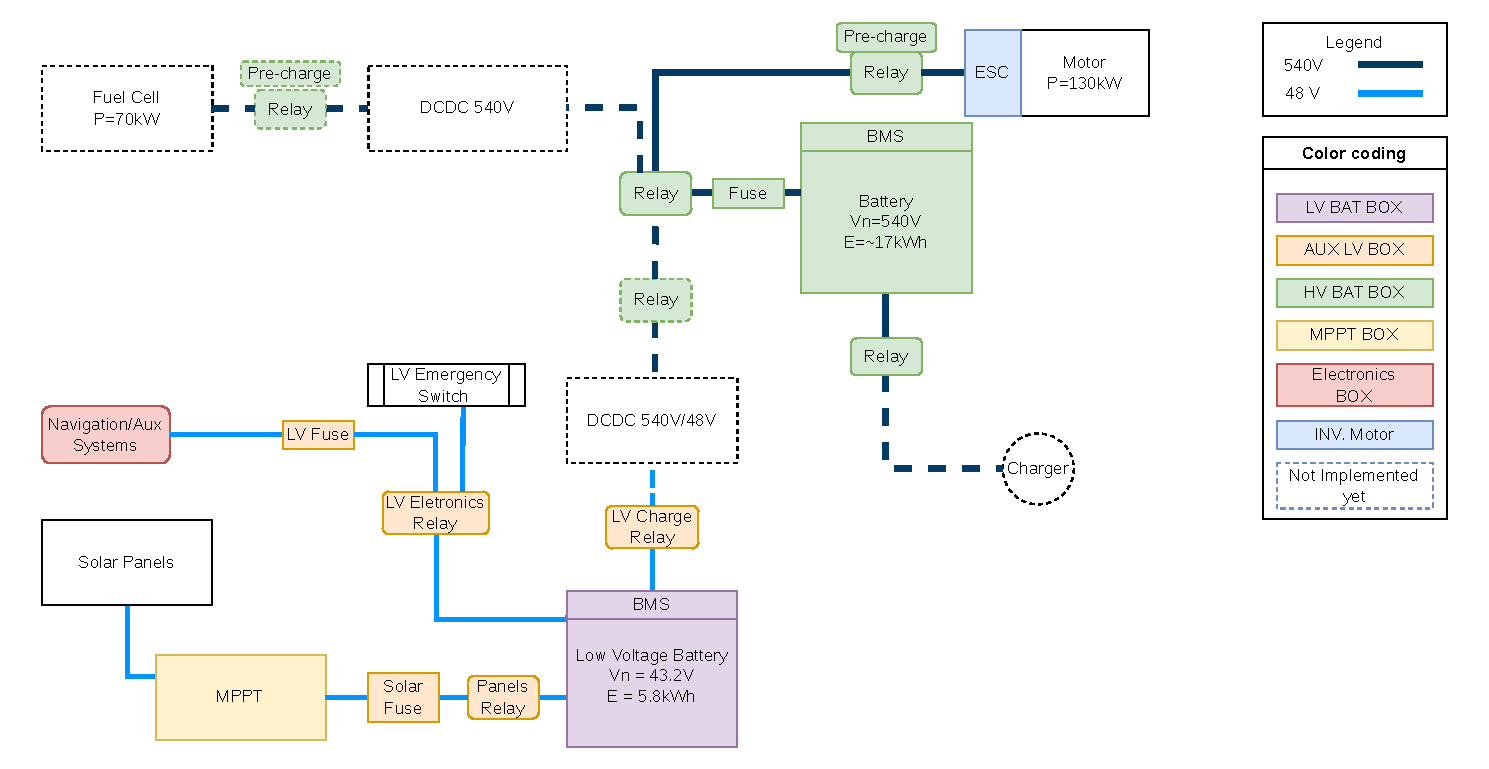
\includegraphics[width=0.90 \textwidth]{Images/System/Sys_diagram.pdf}
    \qquad
    \caption{Simplified electrical schematic of SG01.}
    \label{fig:SG01_sch}
\end{figure}




\section{PV system}

The photovoltaic system of \ac{sg01} was designed to maximize the energy harvested from the available deck area while maintaining reliable operation under the varying environmental conditions encountered in marine applications.

The current installation consists of 140 Maxeon Gen 3 (Me3) photovoltaic cells distributed among ten custom-manufactured solar panels. These panels are connected to four independent \acp{mppt}, as illustrated in Figure~\ref{fig:PV_SG01}. The distribution of panels among the \acp{mppt} was carefully selected to reduce the effects of partial shading, temperature gradients, and non-uniform solar irradiance across the vessel surface. By electrically separating regions with different operating conditions, each \ac{mppt} can independently track the optimal operating point of its associated panels, increasing the overall energy yield.

\begin{figure}[!ht]
    \centering
    \begin{subfigure}{0.49\textwidth}
        \centering
        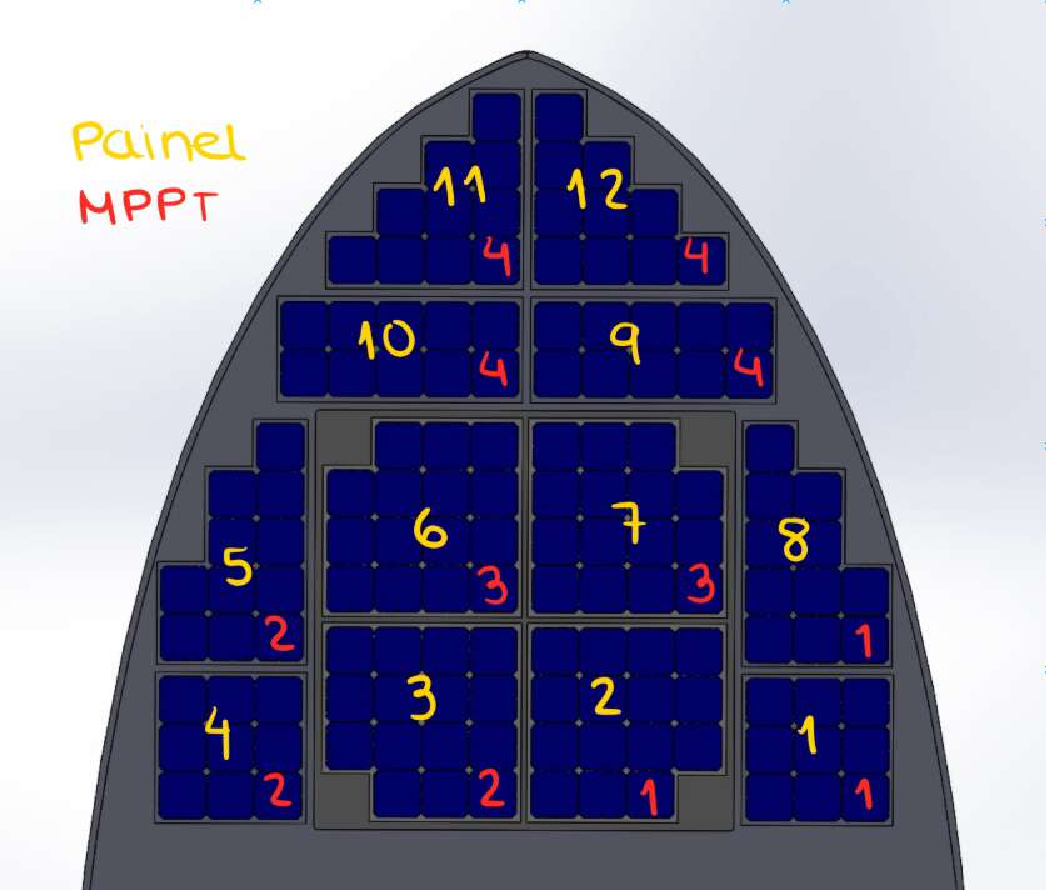
\includegraphics[width=0.99 \textwidth]{Images/System/solar panels.pdf}
        \qquad
        \caption{Distribution of Solar Panels and \ac{mppt} on SG01.}
        \label{fig:PV_SG01}
    \end{subfigure}
    \hfill
    \begin{subfigure}{0.49\textwidth}
         \centering
        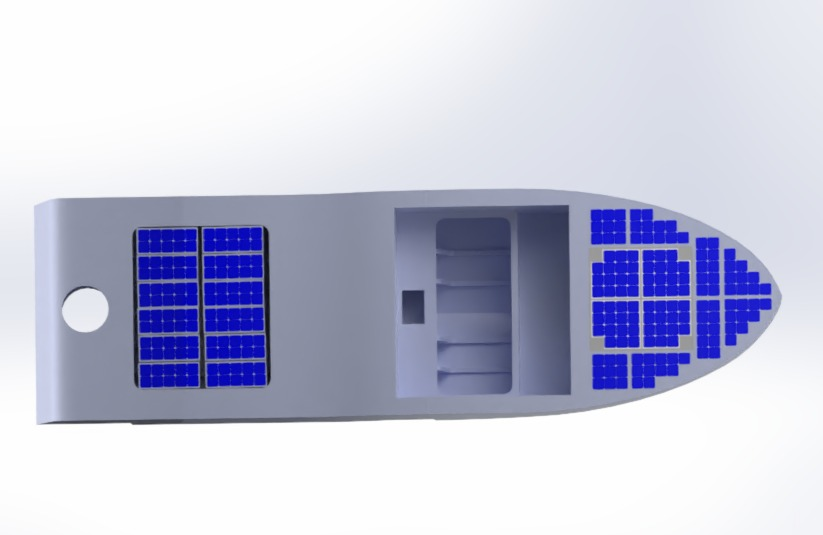
\includegraphics[width=0.99 \textwidth]{Images/System/boat_render.jpeg}
        \qquad
        \caption{Render of São Gabriel 01 with additional solar panels.}
        \label{fig:renderSG01}
    \end{subfigure}
    \caption{Solar panels installation on \ac{sg01}.}
    % \label{fig:}
\end{figure}

Each \ac{pv} cell has an active area of approximately $155.06~\mathrm{cm^2}$, resulting in a total photovoltaic area of $2.171~\mathrm{m^2}$.

Assuming \ac{stc} (irradiance of $1000~\mathrm{W/m^2}$ AND 25ºc), the photovoltaic array is capable of delivering approximately $526.4~\mathrm{W}$ of peak power (theoretical value). 

The \ac{pv} energy is extracted by four commercial Genasun \acp{mppt}, which are grouped in a dedicated \ac{mppt} box. The \acp{mppt} convert the variable voltage produced by the solar panels into a stable charging voltage suitable for the low voltage battery system. This architecture allows each photovoltaic group to operate close to its \ac{mpp}independently, improving energy extraction under non uniform illumination conditions.

To ensure high performance and shape configurability, the photovoltaic modules were manufactured in house using materials selected specifically for marine operation. This process begins by soldering all cells in a module together and then a lamination is performed using vacuum and heat blacks.

Prior to installation, all panels underwent electroluminescence testing to detect manufacturing defects such as microcracks, broken cells, or interconnection failures, Figure~\ref{fig:ilu_test}. These tests were performed before integration into the vessel to ensure that only panels with acceptable electrical and structural integrity were installed. This quality control procedure reduces the likelihood of premature degradation and enables comparison before and after competitions.

\begin{figure}[!ht]
    \centering
    \begin{subfigure}{0.49\textwidth}
        \centering
        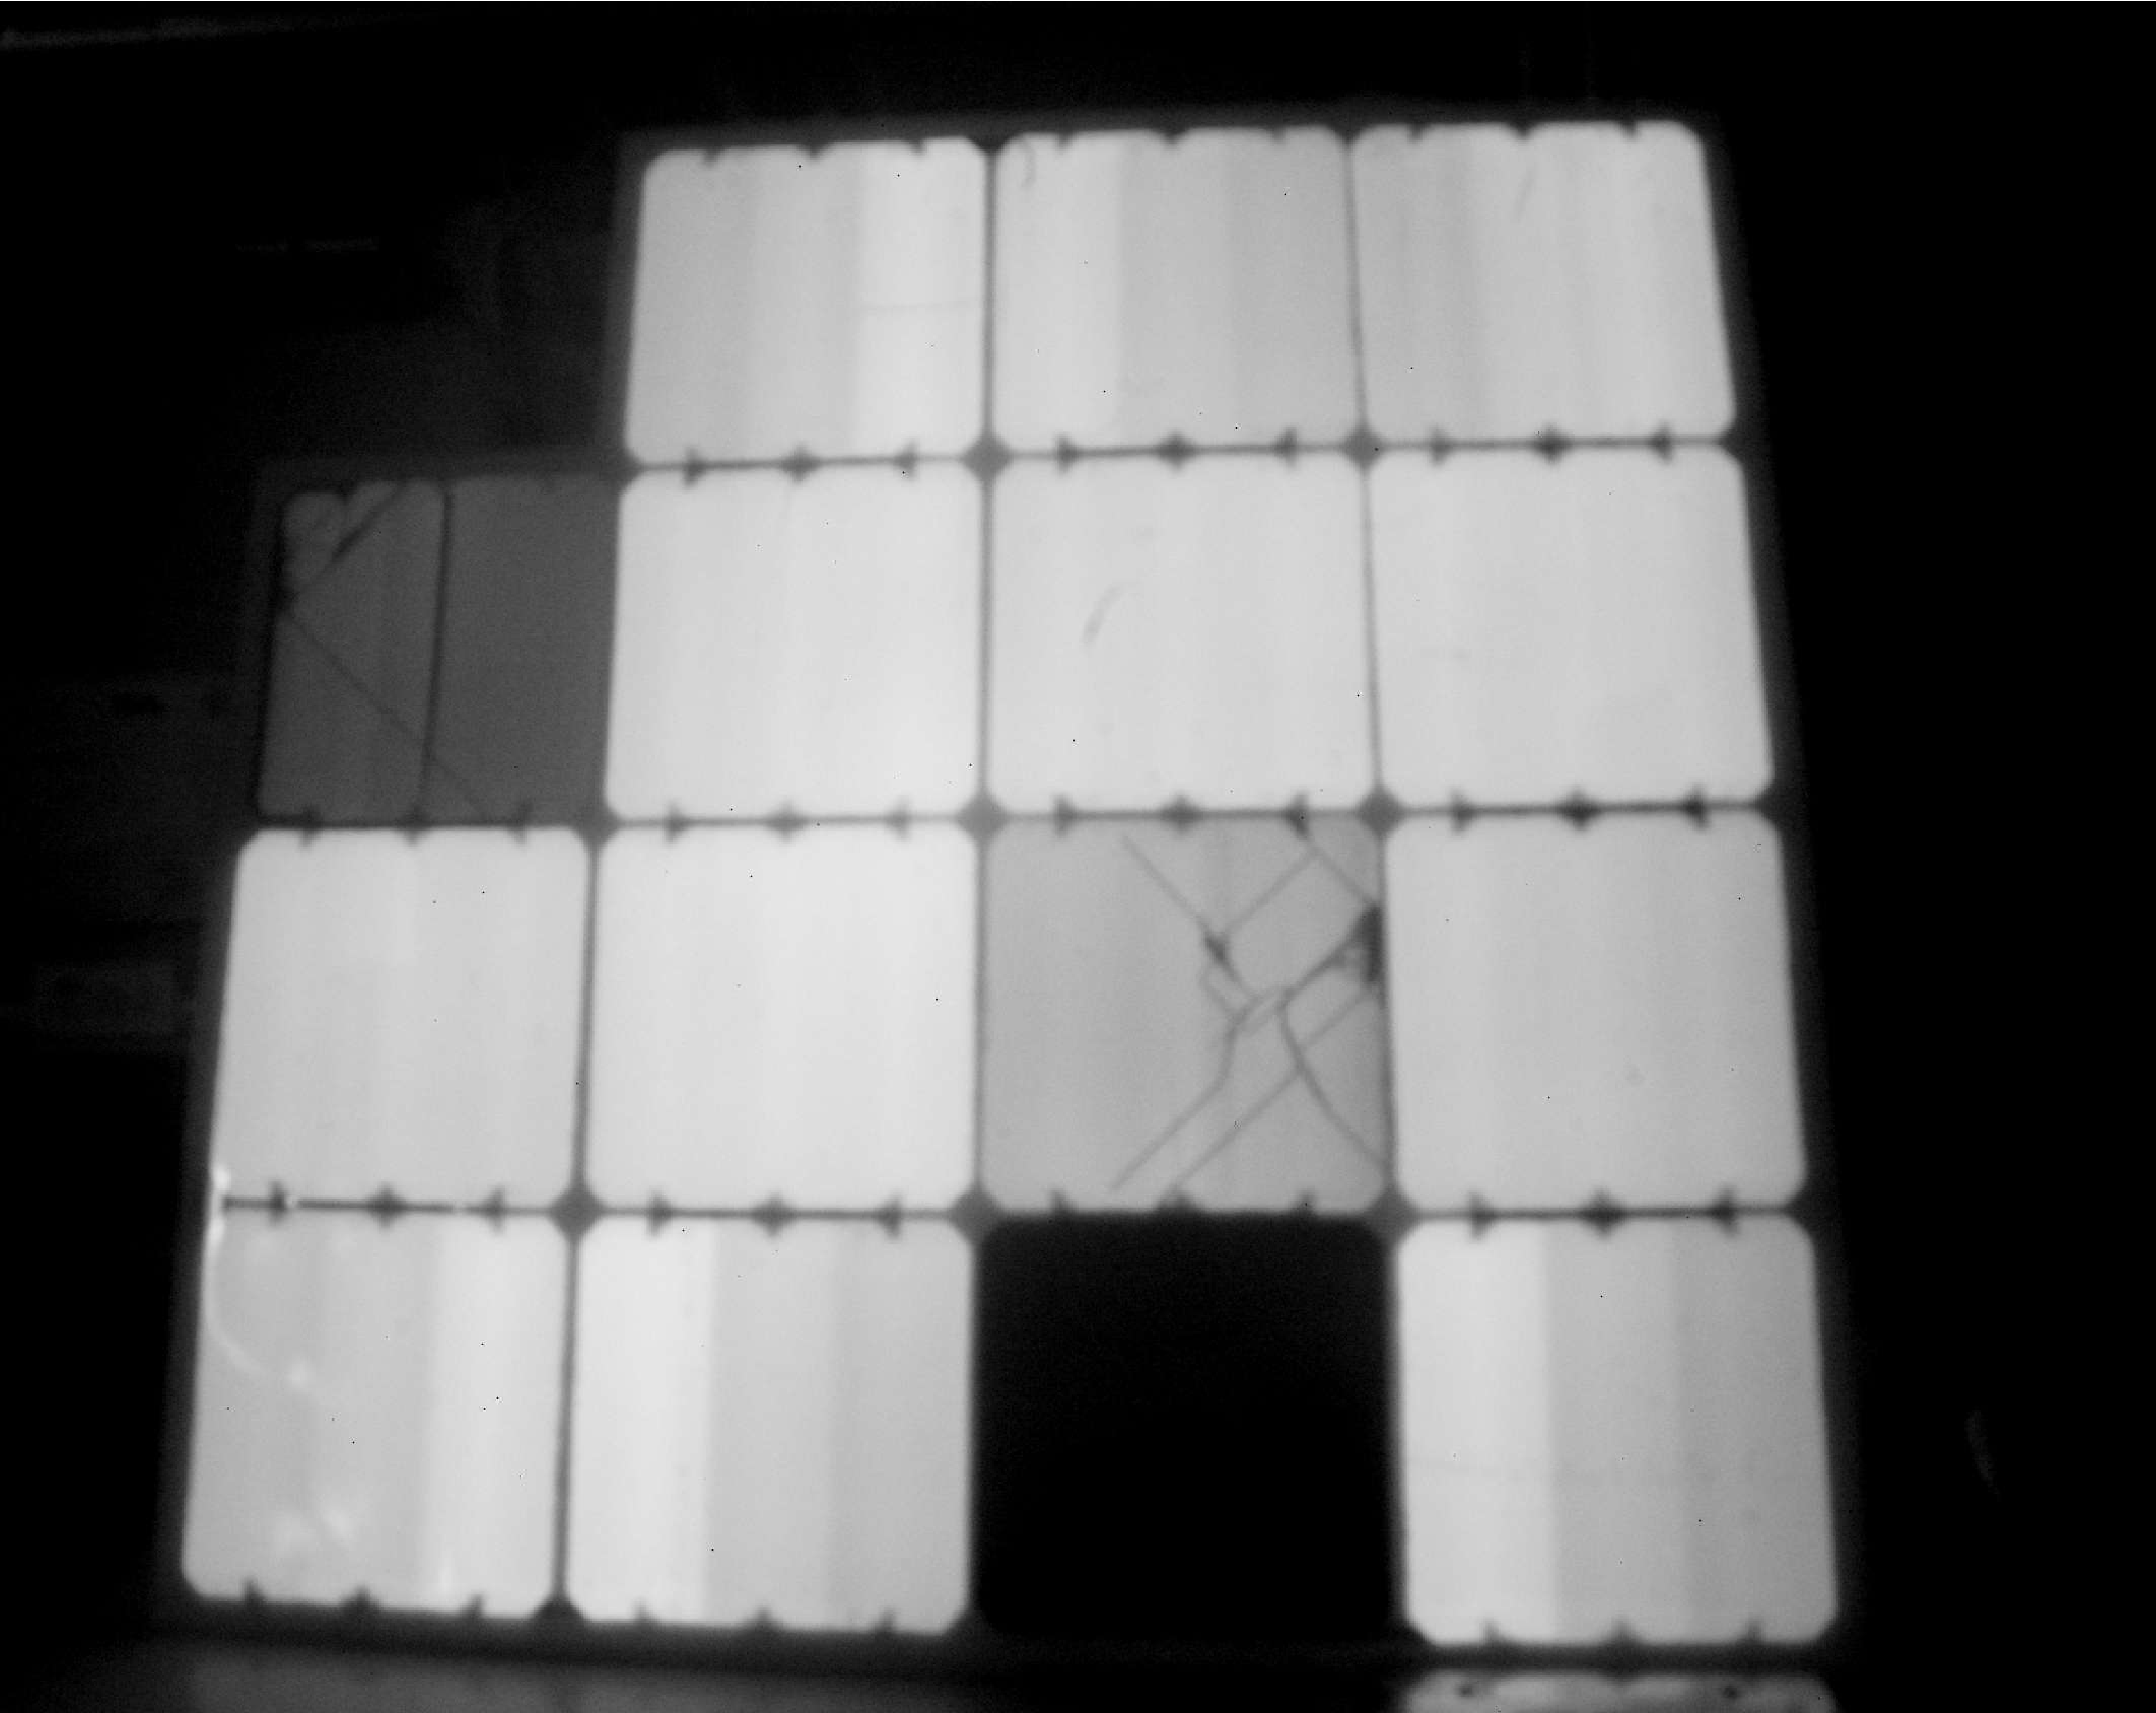
\includegraphics[width=0.8\textwidth]{Images/System/DSC_3873.pdf}
        \caption{Worst results.}
    \end{subfigure}
    \hfill
    \begin{subfigure}{0.49\textwidth}
        \centering
        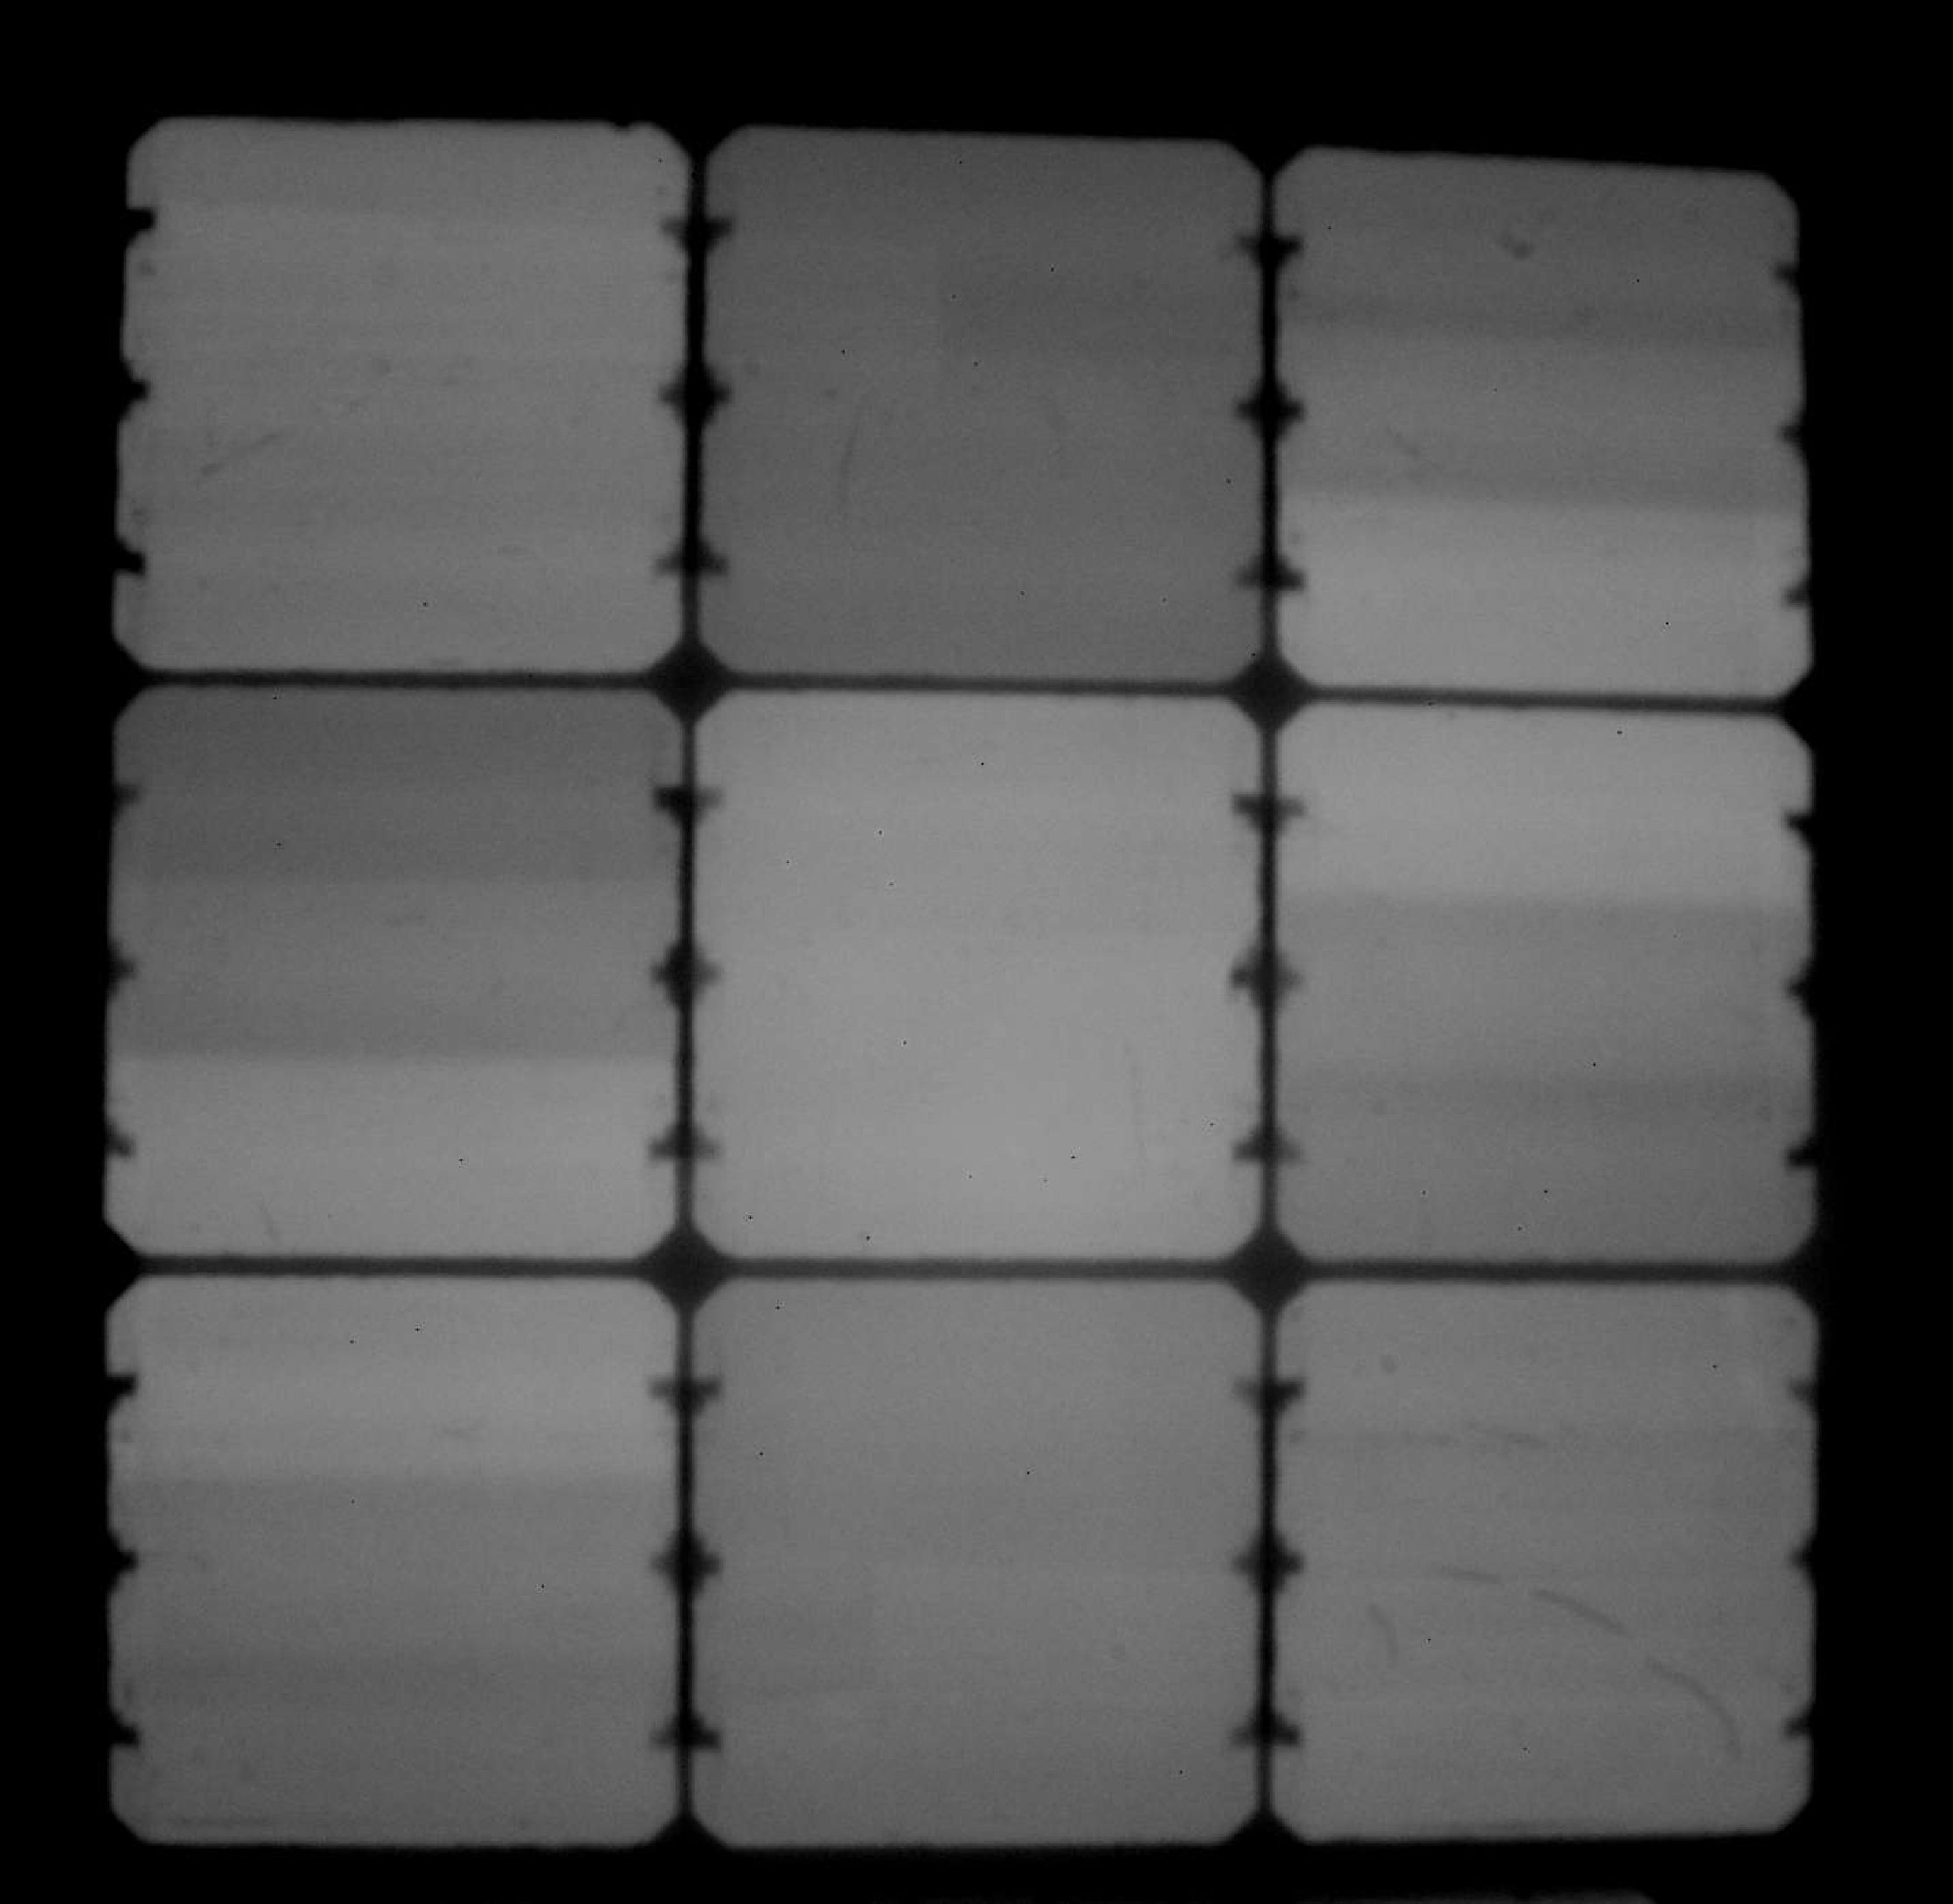
\includegraphics[width=0.65\textwidth]{Images/System/DSC_3887.pdf}
        \caption{Best results.}
    \end{subfigure}
    \caption{Electroluminescence test results.}
    \label{fig:ilu_test}
\end{figure}

Although the current photovoltaic installation already provides a significant contribution to the low-voltage energy budget, additional usable deck area remains available. Figure~\ref{fig:renderSG01} presents a conceptual rendering with supplementary solar panels. Preliminary estimates indicate that the total photovoltaic power could be increased to approximately $977~\mathrm{W}$, almost doubling the currently installed capacity. Such an upgrade would substantially reduce battery charging times and significantly increase the autonomy of the vessel.





\section{Battery}
\label{sec:battery}
In the past years we have been producing our batteries achieving a lower cost and highly customizable solution. In \ac{sg01} we chose lithium-ion cells due to its ease of use and quick assembly. The assembly is done by the members. It begins by placing the cells on plastic holder to increase structural strength, then using a spot welder, the series and parallel connections are made with nickel tabs (Figure~\ref{fig:SG01_battery}). In parallel, some thermistors are place in different locations of the battery to ensuring a precise a robust temperature reading. In the end, the battery is placed in a case with a \ac{bms} and all the necessary connections.

\begin{figure} [!ht]
    \centering
    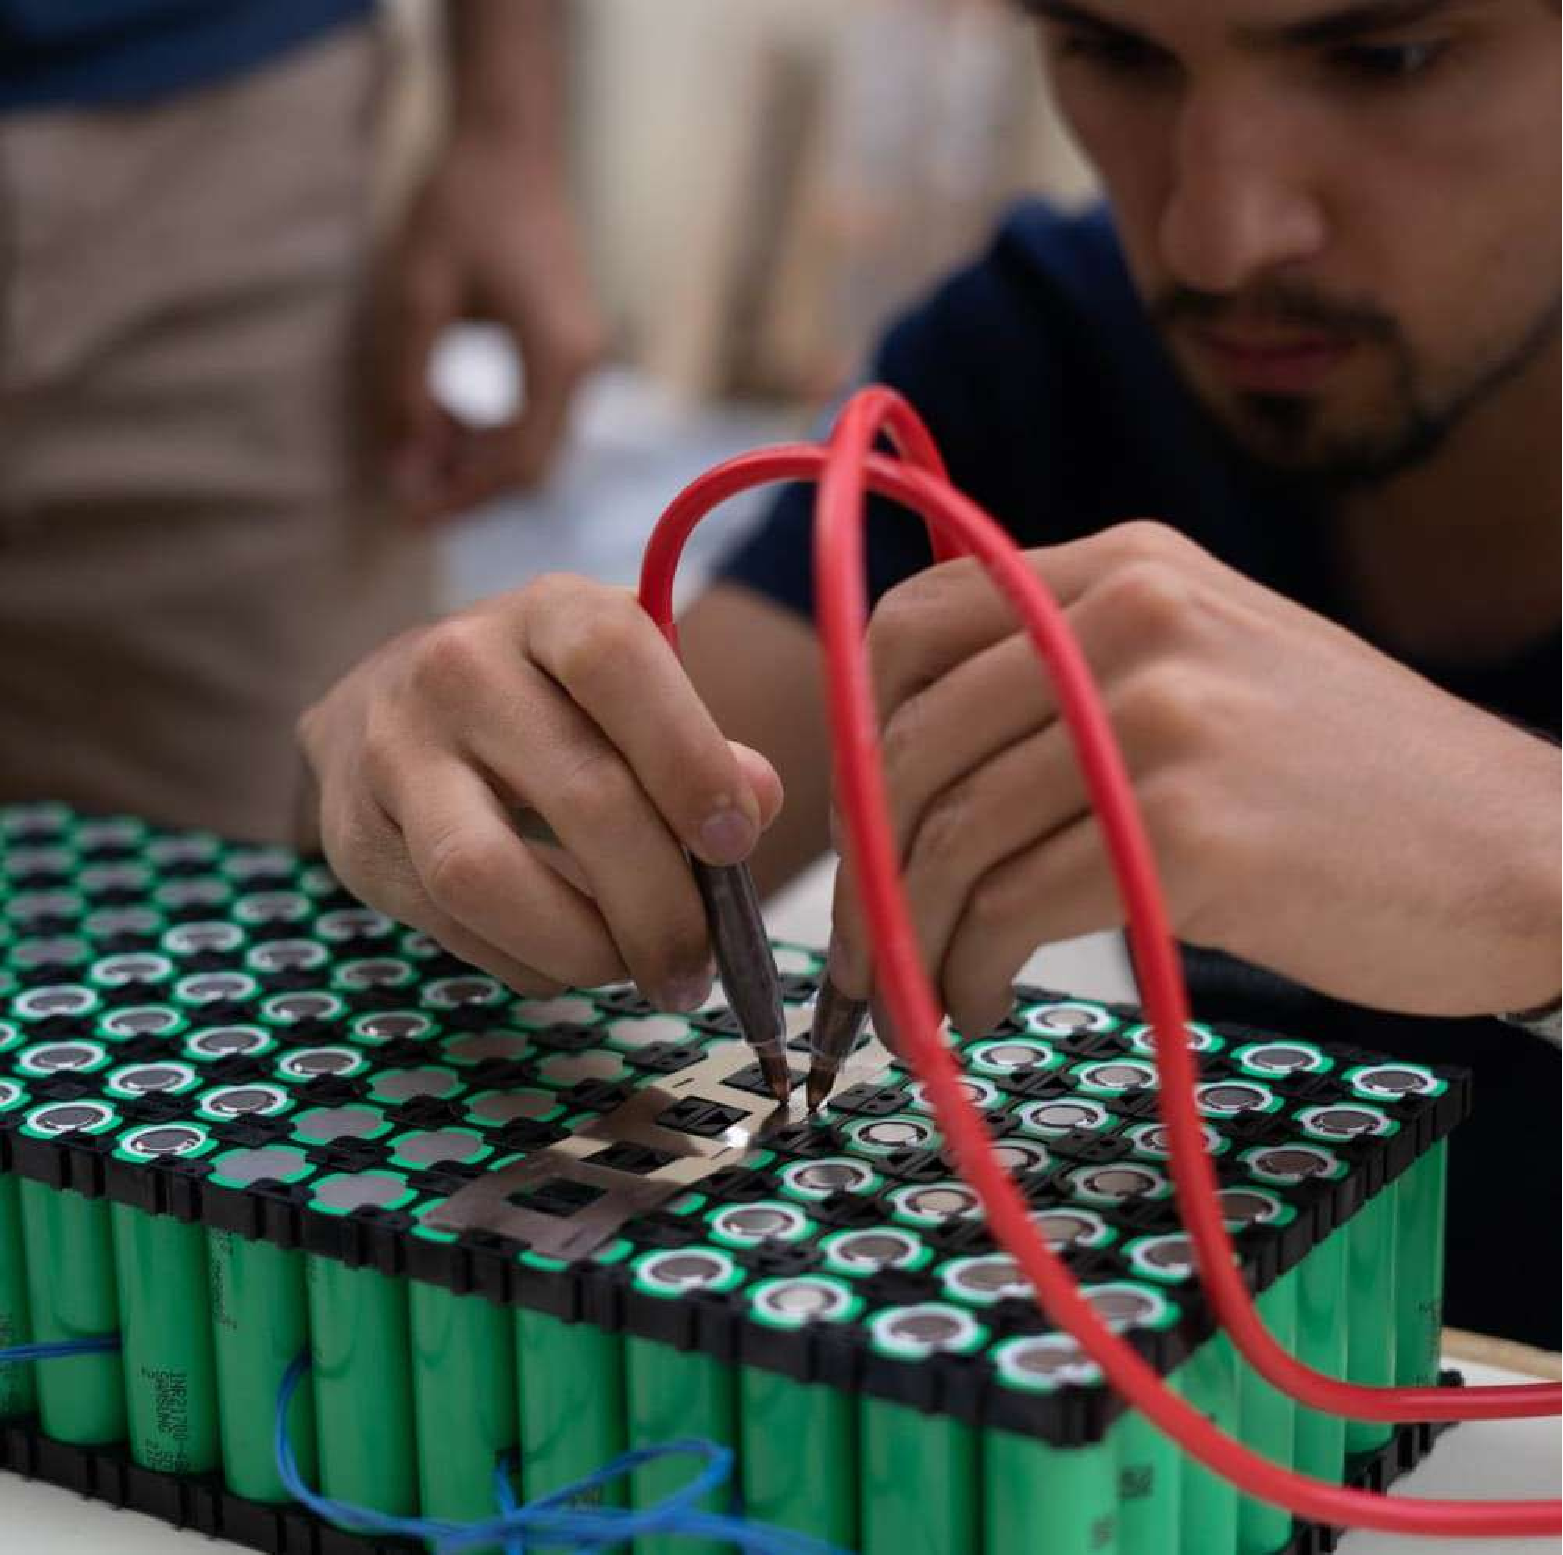
\includegraphics[width=0.50 \textwidth]{Images/System/lv spot welding.pdf}
    \qquad
    \caption{Low voltage battery assembly.}
    \label{fig:SG01_battery}
\end{figure}

The current low voltage battery uses Samsung INR21700-50G cells in a 12s28p configuration. This configuration results in the specifications written in Table~\ref{tab:battery_comparison}.


\begin{table}[htbp]
    \centering
    \caption{\ac{sg01} and \ac{sr03} battery specs.}
    \label{tab:battery_comparison}
    \begin{tabular}{|l|c|c|c|c|}
        \hline
        \textbf{Parameter} & \textbf{Unit} & \textbf{SG01 Battery} & \textbf{SR03 Battery} & \textbf{NAVICTUS Battery}\\ \hline
        Max Voltage & V & 50.4 & 50.4 & 50.4\\ \hline
        Nominal Voltage & V & 43.2 & 43.2 & 43.56\\ \hline
        Min Voltage & V & 30 & 30 & 30\\ \hline
        Configuration & -- & 12s28p & 12s7p & 12s1p \\ \hline
        Number of cells & -- & 336 & 84 & 12\\ \hline
        Energy Capacity & Wh & 5866.56 & 1512 & 223.9 \\ \hline
        Capacity & Ah & 135.8 & 35 & 5.140\\ \hline
        Max charge current & A & 135.8 & 42 & 5.3 \\ \hline
        Cutoff charge current & A & 3.395 & 1.75 & 0.133 \\ \hline
        Max discharge current & A & 271.6 & 175 & 15.9\\ \hline
        Weight & kg & 25.2 & ? & 1\\ \hline
        Internal resistance & m$\Omega$ & 6 & 24 & 192\\ \hline
    \end{tabular}
\end{table}

\ac{sg01} battery was designed for a different vessel which needed a substantial higher capacity. The battery is too heavy, and overall overdimensioned. 

For a more realistic impact analysis, \ac{sr03} battery will be used. This is a much smaller battery with a reasonable capacity for this vessel. It uses Samsung INR21700-50s cells in a 12s7p configuration. This configuration results in the specifications also written in Table~\ref{tab:battery_comparison}.

Additionally, to reduce the time of the charging test another battery is used. This battery was provided by a startup called NAVICTUS and is a 12s1p with INR21700-53G cells from Samsung.

\section{PV System Impact on Autonomy}

With \ac{sg01} battery (5844.56~Wh) and the maximum power that the solar panels can currently provide (526.4~W), the minimum time to fully charge the battery is 11h and 7min (5844.56~Wh / 526.4~W). This is a large time to charge a battery. There are two solutions to this problem: increase the power provided by the solar panels or decrease the battery capacity.

Let's consider the case where we reduced the battery capacity of 1512~Wh which is the capacity of our solar boat (\acs{sr03}) battery. With this change alone the battery is fully charged in 2h and 53min, which is a much more reasonable time. Additionally, if we increase the power provided by the solar panels to 977 W, the battery will be fully charged in 1h and 33min, which is an excellent time to charge a battery.


The charging times are a good to evaluate the \ac{pv} system, but the main goal is to maximize the time on water before full battery discharge. For that lets consider 1000~W of consumption. Considering the original battery it takes 5~h 51~min to fully discharge without solar panels and 12~h 21min with solar panels and approximately 10 days with the additional solar panels. As previously said, this battery is overdimensioned and will be changed in the future.

To get a better idea of the impact of the \ac{pv} system lets consider the battery of \acs{sr03}. This battery takes 1~h and 30~min to fully discharge without solar panels and 3~h 12~min with solar panels and approximately 2 days 18~h with the additional solar panels. 

By reducing the battery capacity and increase the solar panel area, the battery would never need external charging. In another point of view, the low voltage system can drain more power from the battery.



\section{Environmental changes}

In engineering, the term ``fast'', used in the title of this thesis, needs to be associated with a time scale. A process can only be considered fast when compared with another process with a longer characteristic time. Therefore, this section investigates the characteristic time scales associated with variations in the \ac{mpp} caused by environmental changes, with particular emphasis on the oscillatory motion of the vessel and its implications for the required speed of the MPPT algorithm.

When analyzing \ac{mpp} variations, there two main factors: temperature and irradiance. Temperature variations are generally slower than variations in irradiance. Although rapid temperature changes can occur, for example when water comes into contact with the photovoltaic panels, such events are considered unusual during normal operation and are therefore not considered in this analysis. Irradiation on the other hand, can vary more rapidly as the angle of the solar panels changed with the vessel angle, particularly roll and pitch. 

The motion of a vessel subjected to waves can be described as a forced dynamic system. The vessel has characteristic natural frequencies associated with its different modes of motion, including roll, pitch and heave. The response to wave excitation depends on the relationship between the excitation frequency and the corresponding natural frequency of the vessel. In particular, when the excitation frequency approaches a natural frequency, the response amplitude can increase significantly due to resonance. The vessel does not, however, necessarily oscillate at its natural frequency when subjected to excitation at another frequency, the steady state response occurs primarily at the excitation frequency, while the natural frequency determines the dynamic response and its amplitude.

Considering a simplified undamped free oscillation system, the natural frequency of a vessel can be calculated using the natural period Formula~\ref{eq:fundamental period} where $I$ is the mass moment of inertia and $C$ is the restoring stiffness \cite{rao2011mechanical}.

\begin{equation}
    T = 2\pi \sqrt{\frac{I}{C}}
    \label{eq:fundamental period}
\end{equation}

When applied to pitch and roll, the restoring stiffness is given by the mass (m), gravity (g) and metacentric height ($GM_L$ for pitch and $GM_t$ for roll). Since the inertia mass was not given, the equation was further simplified using the radius of gyration in pitch or roll ($k_{yy}$ or $k_{xx}$) which is equivalent to Formula~\ref{eq:radius of gyration}.

\begin{equation}
    k = \sqrt{\frac{I}{m}}
    \label{eq:radius of gyration}
\end{equation}

\begin{equation}
    T = 2\pi \sqrt{\frac{I}{mgGM}} \leftrightarrow T = 2\pi \sqrt{\frac{k_{yy}^2}{gGM_L}}
    \label{eq: natural period}
\end{equation}

For pitch, $k=k_{yy}$ and $GM=GM_L$, whereas for roll, $k=k_{xx}$ and $GM=GM_T$.

This formula is used with results given by the hydrostatic simulations which were provided by \ac{tsb}, where $GM_L$ is $21.515~\mathrm{m}$ and $GM_t$ is $1.867~\mathrm{m}$. Also, the radius of gyration is calculated based on the longitude (L=8~m) and width/beam (B=2.5~m). Based on the International Towing Tank Conference (ITTC) recommendation \cite{ittc_seakeeping_2024}, when the radius of gyration for pitch and roll is unknown a value of 0.25L and 0.35B to 0.40B, respectively, should be used.

Based on the given values, the pitch and roll natural period is 0.8654 and 1.2853 respectively, which is equivalent to 1.1555~Hz and 0.7780~Hz. These values represent a estimative of the natural frequencies of the vessel.

As for the frequency of the waves it has an extensive range and depends on several factors. Studies on this subject show higher energy for waves with 1 to 30 seconds periods which is equivalent to 0.033~Hz to 1~Hz, Figure~\ref{fig:wave by period}.

\begin{figure} [!ht]
    \centering
    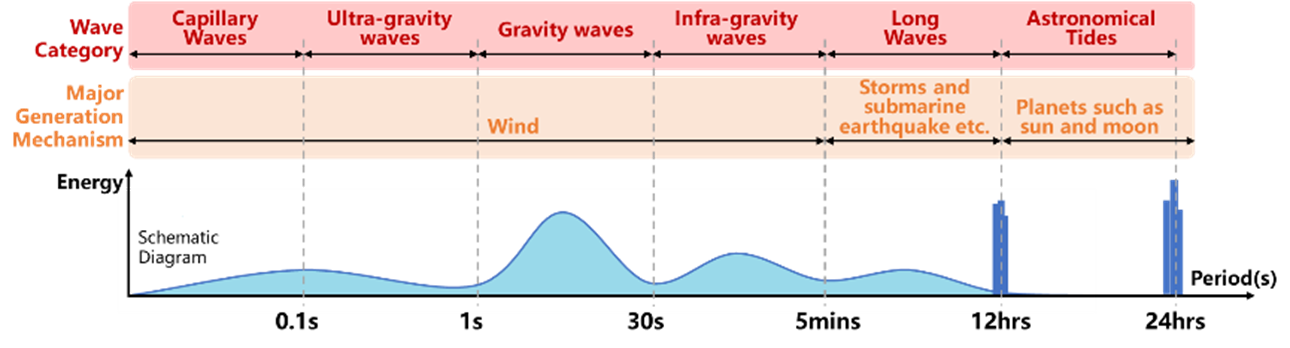
\includegraphics[width=0.90 \textwidth]{Images/System/wave_by_period.png}
    \qquad
    \caption{Classification of waves by period and respective energy \cite{newfrontiers2018}.}
    \label{fig:wave by period}
\end{figure}

The environmental excitation experienced by \ac{sg01} was further investigated using experimental data collected while the vessel was adrift at sea. Ten datasets containing the roll and pitch angles were collected and combined to obtain the frequency domain response shown in Figure~\ref{fig:sg01 wave}. The results show significant spectral components at approximately 0.05~Hz and 0.5~Hz. The lower frequency must be due to the fast winds or transient oscillations, and it is consistent with the local forecast wave period. The higher frequency can be caused by the natural frequency of vessel. The root causes were not investigated further, since it falls outside the scope of this project.

\begin{figure} [!ht]
    \centering
    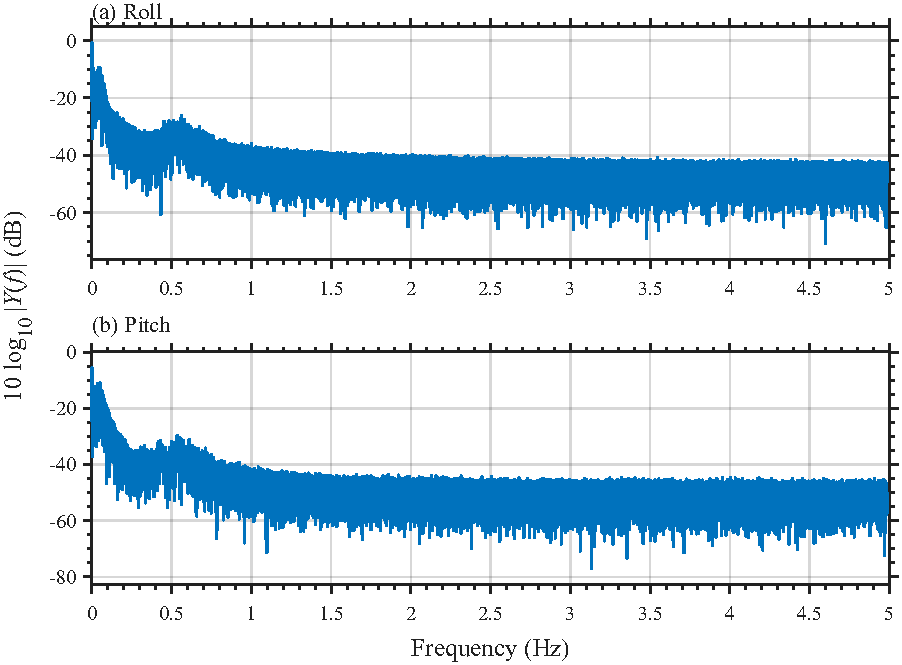
\includegraphics[width=0.90 \textwidth]{Images/System/sg01_osc.pdf}
    \qquad
    \caption{Measured oscillations from \ac{sg01}.}
    \label{fig:sg01 wave}
\end{figure}

Both theoretical and experimental results predict or measure frequency up to 1~Hz. In the context of the \ac{mppt} algorithm, the goal will be a minimum speed of 1~Hz or 1 seconds and a typical speed of more than 2~Hz or 0.5~seconds.

These value will have directly influence on the sampling time as will discuss later. 
% https://geo.libretexts.org/Bookshelves/Oceanography/Introduction_to_Physical_Oceanography_(Stewart)/16%3A_Ocean_Waves/16.4%3A_Ocean-Wave_Spectra

% See Swell Period and hight here https://bigsalty.com/en/weather/forecast/8350/
